\section{Durchführung}
\label{sec:Durchführung}
Der schematische Aufbau für die Aufnahme einer Franck-Hertz-Kurve wurde bereits erläutert und in \autoref{fig:aufbau} dargestellt. Für die praktische Aufnahme der Kurve wurde diese Schaltung zu der in \autoref{fig:aufbau2} dargestellten Schaltung erweitert. 
\begin{figure}[H]
    \centering
    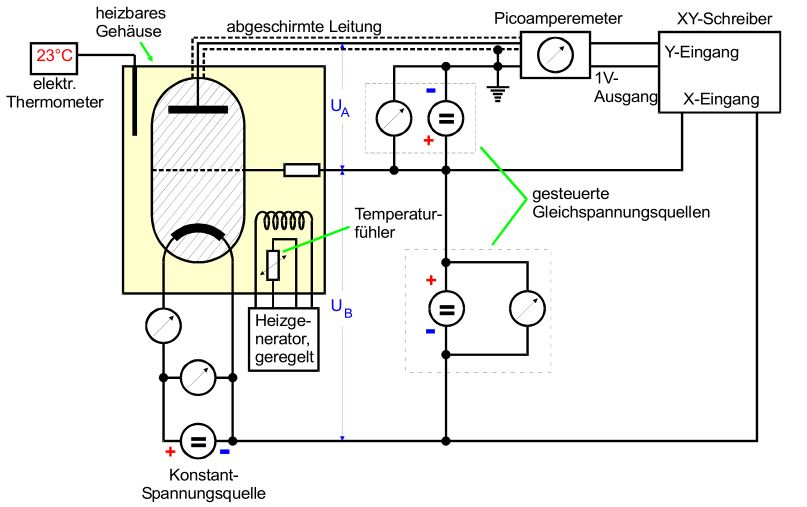
\includegraphics[width=\textwidth]{images/aufbau2.JPG}
    \caption{Schaltung für die Aufnahme einer Franck-Hertz-Kurve. \cite{V601}}
    \label{fig:aufbau2}
  \end{figure}
\noindent
Man benötigt zusätzlich also einen Heizgenerator mit Thermometer und einen XY-Schreiber zum Aufzeichnen der Kurven. Für die Bedienung und das Ablesen werden Gleichspannungsquellen und ein Picoamperemeter genutzt.\\
\\
Zuerst wird die Energieverteilung gemessen. Dazu wird eine konstante Beschleunigungsspannung von $U_\text{B} = \SI{11}{\volt}$ eingestellt, während 
die Bremsspannung erhöht wird.
Dabei zeichnet der XY-Schreiber den Verlauf des Auffängerstroms in Abhängigkeit von der Bremsspannung auf.\\
Diese Messung wird für zwei unterschiedliche Temperaturen durchgeführt. Die erste Messung wird bei einer Temperatur von ungefähr $\SI{20}{\celsius}$
und die zweite Messung in einem Temperaturbereich von $\SI{140}{\celsius}$ bis $\SI{160}{\celsius}$ durchgeführt. Die Temperatur wird dabei mit dem Heizgenerator eingestellt.\\
Abschließend wird die X-Achse skaliert, indem mit dem XY-Schreiber in $\SI{1}{\volt}$-Schritten Markierungen auf das Blatt gesetzt werden.\\ 
\\
Im zweiten Teil der Versuchsdurchführung wird eine Franck-Hertz-Kurve aufgenommen. Hier wird eine konstante Bremsspannung von $U_\text{A} = \SI{1}{\volt}$ eingestellt, während die Beschleunigungsspannung in einem Bereich von $\SI{0}{\volt}$ bis $\SI{60}{\volt}$ variiert wird. Hier werden mehrere Kurven für unterschiedliche Temperaturen innerhalb eines Temperaturintervalls von $T = \SI{160}{\celsius}$ bis $T=\SI{200}{\celsius}$ mit Hilfe des XY-Schreibers aufgenommen. Auch hier muss abschließend die X-Achse skaliert werden.